% Szglab4
% ===========================================================================
%
\chapter{Grafikus felület specifikációja}

\thispagestyle{fancy}

\thispagestyle{fancy}

\section{A grafikus interfész}
A szoftver elindulásakor a játékos egy eltéveszthetetlenül egyszerű menüben fogja találni magát, ahol
választhat hogy hány játékos vegyen részt a játékban. Az egész játék, úgy ahogyan a menü is korunk csempe életérzését fogja tükrözni

\begin{figure}[h]
	\begin{center}
		
\includegraphics[width=5cm]{chapters/chapter11/StapelMenu.png}
		\caption{menu}
		\label{fig:Grafikus}
	\end{center}
\end{figure}

Miután a felhasználó kiválasztotta a játékosok számát a játék elindul. Az egész játék egy panelekre osztott játéktérben fog zajlani, ahol a játékos az egér segítségével tudja majd mozgatni a robotot, illetve csapdákat letenni vele.

\begin{figure}[h]
	\begin{center}
		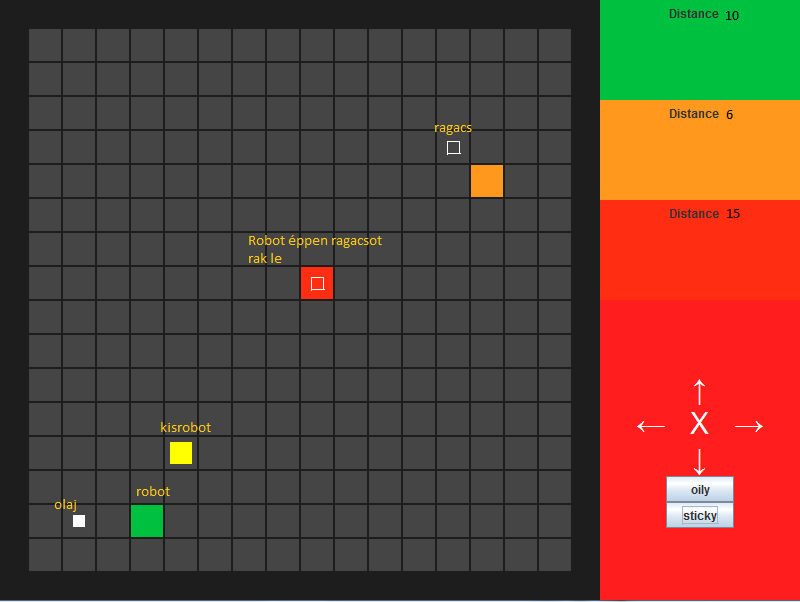
\includegraphics[width=17cm]{chapters/chapter11/StapelInGame.png}
		\caption{játék közben}
		\label{fig:Grafikus}
	\end{center}
\end{figure}


\section{A grafikus rendszer architektúrája}

\subsection{A felület működési elve}
	A Window osztály az egész felület containere, ez egy form egy jobb oldali, és egy bal oldali panelből áll. A bal oldali panel megjeleníthető a GameStartPanel osztály egy példányát, ebben az esetben
	a menü rajzolódik ki. A másik lehetőség hogy a GamePanel egy osztálya jelenik meg a bal oldalon,
	ami egy aktív játékteret ábrázol.
	A jobb oldali panel szintén container. Ez tartalmazza játék közben a felső részében eredménypanelt, illetve az alsó részében a vezérlő panelt.
	Indításnál a gamestartpanel a gombot action listenere is egyben. Ha a user klikkel, akkor gamecontroller elindítja a játékot, a megadott számú robottal, innentől a controller panel veszi át az input controller szerepét. 
	A controllerpanel listenerjei a gamecontroller függvényeit hívja meg. Léptetésnél a robotStep fogja léptetni a robot, a modellben elindítani a folyamatokat, és továbbadni a vezérlést a soron következő robotnak.
	
	Minden kirajzolandó játékbeli objektumhoz, tehát a Robot, Pálya, Ragacs és Olajfolt tartozik egy View Osztály is. Ez a View osztály végzi el az egyes elemek kirajzolását. A következő a folyamat: A modell változik a user input hatására, miután a model updatelődött a GamePanel újrarajzolódik, ami cserébe meghívja a View objektumot és a Panelek paintComponent metódusát, ami újrarajzolja a játékteret.
	 
	Az grafikus Architektura pull modellre épül, mert minden lépés után a grafikus interface lekéri a modellből a változásokat, és aktualizálja a grafikus interfacet.
	\clearpage
\subsection{A felület osztály-struktúrája}


\begin{figure}[h]
	\begin{center}
		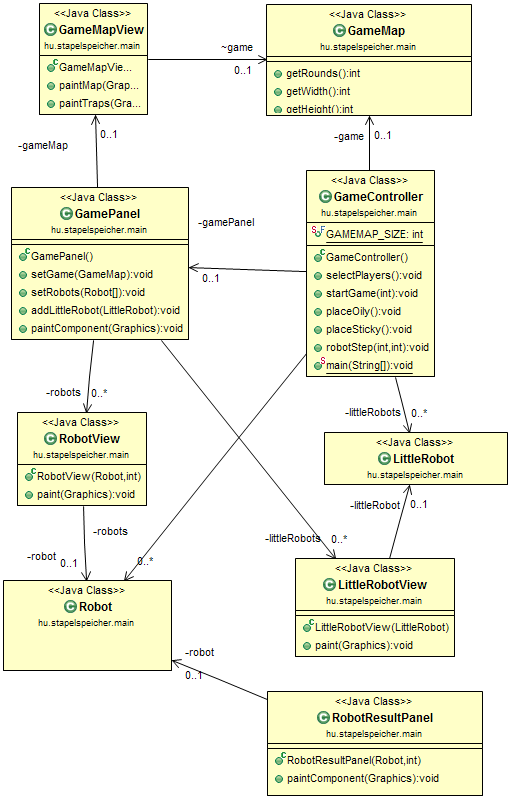
\includegraphics[width=11cm]{chapters/chapter11/StapelGrafUML1.png}
		\caption{Grafikus UML első fele}
		\label{fig:Grafikus}
	\end{center}
\end{figure}

\clearpage
\begin{figure}[h]
	\begin{center}
		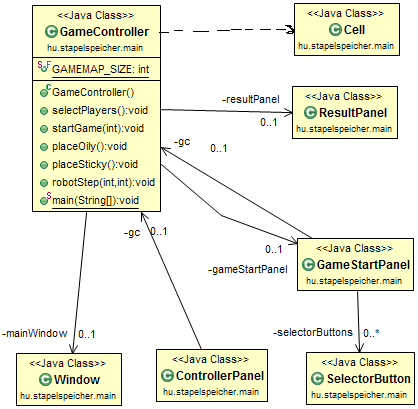
\includegraphics[width=14cm]{chapters/chapter11/StapelGrafUML2.png}
		\caption{Grafikus UML második fele}
		\label{fig:Grafikus}
	\end{center}
\end{figure}






\section{A grafikus objektumok felsorolása}

\subsection{GameController}
\begin{itemize}
	\item Felelősség\newline
	Létrehozza a játékot, az egész játék irányításáért felelős osztály. A generált pályához létrehoz annyi robotot, ahányat az elején kiválasztanak a felhasználók. A kör léptetése is itt történik.
	
	\item Attribútumok\newline

	\begin{itemize}
		\item -mainWindow: Window: 
		\item -game: GameMap:
		\item -gameStartPanel: GameStartPanel:
		\item -resultPanel: ResultPanel: Az eredményjelző panel.
		\item -players: int: A játékosok száma.
		\item -robots[]: Robot: A robotokat tároló objektum.
		\item -littleRobots: ArrayList<LittleRobots>: A kisrobotokat tároló objektum. 
		\item -randomGenerator: Random: Random generátor.
		\item -currentRobot: int: Az épp aktuálisan kijelölt robot.
		\item -robotsAlive: int: Az életben lévő robotok száma.
		\item -gamePanel: GamePanel: 
		\item \underline{+GAMEMAPSIZE: int}: A pálya méretét eltároló konstans.
		\item \underline{-OILY: int}: Az olajfoltok száma.
		\item \underline{-STICKY: int}: A ragacsfoltok száma.
		\end{itemize}
	\item Metódusok\newline
	\begin{itemize}
		\item +startGame(int players): void: Létrehozza a pályát, beállítja a robotok és a kisrobotok számát. 
		\item +selectPlayers(): void: Létrehozza a játékhoz szükséges paneleket.
		\item -endGame(): void: A játék végét jelző eseményt hajtja végre.
		\item -nextRound(): void: Csökkenti a körök számát és lépteti a kisrobotokat, valamint létrehoz újabb kisrobotokat minden 3. körben.
		\item +placeOily(): void: Olajfolt elhelyezése. 
		\item +placeSticky(): void: Ragacsfolt elehelyezése.
		\item +robotStep(int x, int y): Lépteti a robotokat.
		\item \underline{+main(String args[]): void:} A játék Main függvénye.
	\end{itemize}
\end{itemize}

\subsection{GameMapView}
\begin{itemize}
	\item Felelősség\newline
	A pályát kirajzoló osztály. Kirajzolja a négyzetrácsos területet, ezen a ragacsokat és az oljafoltokat.

	\item Attribútumok\newline
	\begin{itemize}
		\item game: GameMap: 
		\item \underline{+BORDERWIDTH: int}:
		\item \underline{+CELLSIZE: int}:
		\item \underline{+CELLGAP: int}:
	\end{itemize}
	\item Metódusok\newline
	\begin{itemize}
		\item +GameMapView(GameMap g): Az osztály konstruktora.
		\item +paintMap(Graphics g): void: A pályát rajzolja ki, amelyen majd a játék zajlani fog.
		\item -paintOily(Graphics g, int x, int y): void: Bizonyos cellákra olajfoltot rajzol ki.
		\item -paintSticky(Graphics g, int x, int y): void: Bizonyos cellákra ragacsfoltot rajzol ki.
		\item +paintTraps(Graphics g): void: A csapdákat kirajzoló függvény, meghívja a paintOily és paintSticky metódusokat.
	\end{itemize}
\end{itemize}

\subsection{RobotView}
\begin{itemize}
	\item Felelősség\newline
	A robotok megjelenítése a felelőssége.
	
	\item Attribútumok\newline
	\begin{itemize}
		\item \underline{+robotColors[]: Color}: A robotok színeit tartalmazza, konstans értékek. 
		\item -robot: Robot: Robot objektum.
		\item -colorIndex: int: A robothoz hozzárendelendő színek indexei a tömbben.
	\end{itemize}
	\item Metódusok\newline
	\begin{itemize}
		\item +RobotView(Robot r, int i): Az osztály konstruktora.
		\item +paint(Graphics g): void: A robotok tényleges kirajzolása.
	\end{itemize}
\end{itemize}

\subsection{LittleRobotView}
\begin{itemize}
	\item Felelősség\newline
	A kisrobotok megjelenítése a felelőssége.

	\item Attribútumok\newline
	\begin{itemize}
		\item littleRobot: LittleRobot: Egy kisrobot objektum.
		
	\end{itemize}
	\item Metódusok\newline
	\begin{itemize}
		\item +LittleRobotView(LittleRobot lr): Az osztály konstruktora.
		\item +paint(Graphics g): void: A kisrobotok tényleges kirajzolása.
	\end{itemize}
\end{itemize}

\subsection{Window}
\begin{itemize}
	\item Felelősség\newline
	Az egész felület containere, egy jobboldali és egy baloldali panelből áll.
	\item Ősosztályok\newline

		JFrame $\rightarrow$ Window

	\begin{itemize}
		\item \underline{+WINDOWSIZEX: int}: Az ablak szélessége, konstans
		\item \underline{+WINDOWSIZEY: int}: Az ablak magassága, konstans
		\item -leftPanel: JPanel: Baloldali panel.
		\item -rightPanel: JPanel: Jobboldali panel.
		\item -resultPanel: JPanel: Az eredményeket megjelenítő panel.
		\item -controllerPanel: JPanel: Az iránytó panel.
	\end{itemize}
	\item Metódusok\newline
	\begin{itemize}
		\item +Window(): Az osztály konstruktora. Beállítja az ablak méretét és az elrendezését
		\item +setLeftPanel(JPanel panel): void: Beállítja a baloldali panelt, kirajzolja az ablka bel oldalára.
		\item +setResultPanel(JPanel panel): void: Beállítja az eredmény panelt, a jobb oldali panel közepén helyezi el.
		\item +setControllerPanel(JPanel panel): void: Az irányító panelt állítja be, a jobboldali panel aljára helyezi el.
	\end{itemize}
\end{itemize}

\subsection{GamePanel}
\begin{itemize}
	\item Felelősség\newline
	Egy aktív játékteret ábrázoló panel, A Window osztály container bal oldala. A modell megváltozása (user input hatására) után a GamePanel mindig újrarajzolódik, s meghívja a kirajzoló objektumokat.
	\item Ősosztályok\newline
		JPanel $\rightarrow$ GamePanel
	\item Attribútumok\newline
	\begin{itemize}
		\item -gameMap: GameMapView:
		\item -robots[]: RobotView: Robotokat megjelnítő objektum.
		\item -littleRobots: ArrayList<LittleRobotView>: Kisrobotokat megjelenítő objektum. 
	\end{itemize}
	\item Metódusok\newline
	\begin{itemize}
		\item +GamePanel(): A GamePanel konstruktora, beállítja a panel méretét és hátterét is.
		\item +setGame(GameMap g): void: Létrehoz egy új GameMapView objektumot.
		\item +setRobots(Robot robots[]): RobotView objektumot hoz létre, ami majd megjeleníti a robotokat.
		\item +addLittleRobot(LittleRobot lr): void: Kisrobotokat megjelenítő objektumot hoz létre.
		\item +paintComponent(Graphics g): void: Meghívja a komponenseket (robot, kisrobot, csapdák) megrajzoló függvényeket.
	\end{itemize}
\end{itemize}

\subsection{ResultPanel}
\begin{itemize}
	\item Felelősség\newline
	Az eredményeket eltároló panel. Megjeleníti a a robotokhoz tartozó távolságokat egyenként.
	\item Ősosztályok\newline
		JPanel $\rightarrow$ ResultPanel
		
		\item Metódusok\newline
		\begin{itemize}
			\item +ResultPanel(Robot robots[]): Az osztály konstruktora. Beállítja a panel hátterét és elrendezését, majd a panelhez rendelődik a robotok eredményei, amelyek külön panelek.
		\end{itemize}
	\end{itemize}
	
\subsection{RobotResultPanel}
\begin{itemize}
	\item Felelősség\newline
	A robotok eredményeit egyenként kiíró panelek.
	\item Ősosztályok\newline

		JPanel $\rightarrow$ RobotResultPanel
		
		\item Attribútumok\newline
		\begin{itemize}
			\item -robot: Robot: Robot objektum.
			\item -distancePanel: JPanel: A távolságot megjelenítő panel.
			\item -xPanel: JPanel: 
			\item -yPanel: JPanel: 
			\item -oilyPanel: JPanel: Az robot rendelkezésére álló olajfoltok számát megjelenítő panel.
			\item -stickyPanel: JPanel: Az robot rendelkezésére álló olajfoltok számát megjelenítő panel.
			\item distanceValueLabel: JLabel: A megett távolságot tartalmazó szöveg.
		\end{itemize}
		\item Metódusok\newline
		\begin{itemize}
			\item +RobotResultPanel(Robot r, int i): Az osztály konstruktora. Beállítja az elrendezést, és a robotoknak megfelelő színeket. Hozzáadja a distancePanelt.
			\item +paintComponent(Graphics g): void: Lekéri az aktuálisan megtett távolságot a robottól, s ezt megjeleníti.
		\end{itemize}
	\end{itemize}
	
\subsection{SelectorButton}
\begin{itemize}
	\item Felelősség\newline
	A JButton-t egészíti ki, hogy választógombként lehessen használni.
	\item Ősosztályok\newline
		JButton $\rightarrow$ SelectorButton
	\item Attribútumok\newline
	\begin{itemize}
		\item -id: int: A gomb ID-ja.
	\end{itemize}
	\item Metódusok\newline
	\begin{itemize}
		\item +SelectorButton(int id): Az ostály kontsruktora.
		\item +getID: int: Lekér az ID-t.
	\end{itemize}
\end{itemize}

\subsection{Cell}
\begin{itemize}
	\item Felelősség\newline
	A pályát felépítő elemet megvalósító osztály, melynek felelőssége a rajta lévő objektumok interakcióinak lekezelése.
	\item Attribútumok\newline
	\begin{itemize}
		\item -actors: List<ActiveObject>: A cellán lévő robotok.
		\item -trap: Trap: A cellán lévő csapda
		\item -pos: Position: A cella koordinátája
		\item -map: GameMap: A játék mappa
	\end{itemize}
	\item Metódusok\newline
	\begin{itemize}
		\item +getAOsForTest():List<ActiveObject>: Kilistázza a robotokat
		\item +getTrapForTest():Trap: Megadja milyen csapda van a cellán
		\item +getPositionForTest():Position: Megadja a cella pozícióját
		\item +setPosition(Position pos): Beállítja a cella pozícióját
		\item +setMap(GemaMap m): Beállítja a pályát
		\item +add(ActiveObject ao): Hozzáad egy robotot a cellához
		\item +add(Trap t): Hozzáad egy csapdát a cellához
		\item +getCellFromHere(Position p):Cell: Megadja a vektornyi távolságra lévő cellát
		\item +remove(ActiveObject ao): Elvesz egy robotot a celláról
		\item +isEmpty():boolean: Megadja hogy üres-e a cella
		\item +getDistanceFromCell(Cell c):double: Megadja két cella távolságát
		\item +getFreeNeighbouringCell():Cell: Megad egy szabad szomszédos cellát
		\item +getNearestTrapRelativePosition():Position: Megadja a legközelebbi csapda relatív pozícióját
		\item +removeTrap(): Eltávolítja a csapdát a celláról
	\end{itemize}
\end{itemize}

\subsection{GameStartPanel}
\begin{itemize}
	\item Felelősség\newline
	A játék elején megjelenő menüt megvalósító osztály
	\item Ősosztályok\newline
	JPanel $\rightarrow$ GameStartPanel
	\item Attribútumok\newline
	\begin{itemize}
		\item -selectorButton: SelectorButton: Egy választógomb.
		\item -playerLabel: JLabel: A panel felirata
		\item -players: int: játékosok száma
		\item -gc: GameController: a játék irányítója
		\item \underline{selectorButtonColors[]}: Color: A gombok színei
	\end{itemize}
	\item Metódusok\newline
	\begin{itemize}
		\item +GameStrtPanel: Konstruktor
		\item +mouseClicked(MouseEvent arg0): Klikkelés
		\item +mouseEntered(MouseEvent event): Egér a gombra került
		\item +mouseExited(MouseEvent event): Az egér elhagyta a gombot
		\item +mousePressed(MouseEvent arg0): Az egeret lenyomták a gombon
		\item +mouseReleased(MouseEvent arg0): Az egeret elengedték a gombról
	\end{itemize}
\end{itemize}

\subsection{LittleRobot}
\begin{itemize}
	\item Felelősség\newline
	A takarító robotot megvalósító osztály, felelőssége a pályán való mozgás a legközelebbi foltok fele és azok feltakarítása.
	\item Attribútumok\newline
	\begin{itemize}
		\item -state: LittleRobotState: A robot állapota takarít/nem takarít/eltérített
		\item -dazedCounter: int: Az eltérítés számlálója
		\item -cleaningCounter: int: A takarítás számlálója
		\item -currCell: Cell: A cella amin elhelyezkedik
		\item -alive:boolean: A robot él vagy nem
	\end{itemize}
	\item Metódusok\newline
	\begin{itemize}
		\item +isAlive():boolean: Megadja, hogy a robot él-e még
		\item +getDazedCounterForTest():int: DazedCounter getterje
		\item +getCleaningCounterForTest():int: CleaningCounter getterje
		\item +getStateForTest():int: State getterje
		\item +startCleaningIfNeeded(): Ha szükséges a robot megkezdi a takarítást
		\item +setState(): A state settere
		\item +stepOn(ActiveObject ao): A kisrobotra való lépéskor elvégzi az ütköztetést
		\item +oilyEffect(): Az olaj hatásának felülírása
		\item +stickyEffect(): A ragacs hatásának felülírása
		\item +collideWithRobot(Robot other): Robottal való ütközést valósítja meg
		\item +die(): A kisrobot eltávolítását végzi el
		\item +setCell(Cell c): Beállít egy cellát a kisrobotnak
		\item +step(): Lépteti a kisrobotot
		\item +getCell():Cell: A kisrobot cellájának gettere
		\item +collideWithLittleRobot(LittleRobot other): Kisrobottal való ütközést végzi el
\end{itemize}
\end{itemize}

\subsection{LittleRobot}
\begin{itemize}
	\item Felelősség\newline
	A takarító robotot megvalósító osztály, felelőssége a pályán való mozgás a legközelebbi foltok fele és azok feltakarítása.
	\item Attribútumok\newline
	\begin{itemize}
		\item -velocity: Position: a robot sebességvektora
		\item -oily: boolean: A robot olajos-e
		\item -stickynum: int: A robot ragacskészletének száma
		\item -oilyNum: int: A robot olajkészletének száma
		\item -distance: int: A robot által megtett távolság
		\item -currCell: Cell: A cella amin elhelyezkedik
		\item -alive:boolean: A robot él vagy nem
	\end{itemize}
	\item Metódusok\newline
	\begin{itemize}
		\item +isAlive():boolean: Megadja, hogy a robot él-e még
		\item +getVelocityForTest(): Position: a velocity gettere
		\item +getStickyForTest(): int: a stickyNum gettere
		\item +getOilyForTest(): int: az oilyNum gettere
		\item +Robot(int stickyNum, int oilyNum): Konstruktor, beállítja a készleteket
		\item +placeSticky(): Elhelyez egy ragacsfoltot azon a cellán amin a robot helyezkedik el
		\item +placeOily(): Elhelyez egy olajfoltot azon a cellán amin a robot helyezekdik el
		\item +addVelocity(Position p): Növeli a robot sebességét a megadott vektorral
		\item +oilyEffect(): Az oljara lépéskor beállítja a robot oily tulajdonságát
		\item +stickyEffect(): A ragac
		\item +stepOn(ActiveObject ao): A robotra való lépéskor elvégzi az ütköztetést
		\item +oilyEffect(): Az olaj hatásának felülírása
		\item +stickyEffect(): A ragacs hatásának felülírása
		\item +collideWithRobot(Robot other): Robottal való ütközést valósítja meg
		\item +die(): A kisrobot eltávolítását végzi el
		\item +setCell(Cell c): Beállít egy cellát a robotnak
		\item +step(): Lépteti a robotot
		\item +getCell():Cell: A robot cellájának gettere
		\item +getDistance():int: a robot distance gettere
		\item +collideWithLittleRobot(LittleRobot other): Kisrobottal való ütközést végzi el
	\end{itemize}
	\end{itemize}

\comment{Az új osztályok felsorolása. Az régi osztályok közül azoknak a felsorolása, ahol változás volt. Ezek esetén csak a változásokat kell leírni.}

\subsection{Osztály1}
\begin{itemize}
\item Felelősség\newline
\comment{Mi az osztály felelőssége. Kb 1 bekezdés. Ha szükséges, akkor state-chart is.}
\item Ősosztályok\newline
\comment{Mely osztályokból származik (öröklési hierarchia)\newline
Legősebb osztály $\rightarrow$ Ősosztály2 $\rightarrow$ Ősosztály3...}
\item Interfészek\newline
\comment{Mely interfészeket valósítja meg.}
\item Attribútumok\newline
\comment{Milyen attribútumai vannak}
\begin{itemize}
\item attribútum1: attribútum jellemzése: mire való, láthatósága (UML jelöléssel), típusa
\item attribútum2: attribútum jellemzése: mire való, láthatósága (UML jelöléssel), típusa
\end{itemize}
\item Metódusok\newline
\comment{Milyen publikus, protected és privát  metódusokkal rendelkezik. Metódusonként precíz leírás, ha szükséges, activity diagram is  a metódusban megvalósítandó algoritmusról.}
\begin{itemize}
\item int foo(Osztály3 o1, Osztály4 o2): metódus leírása, láthatósága (UML jelöléssel)
\item int bar(Osztály5 o1): metódus leírása, láthatósága (UML jelöléssel)
\end{itemize}
\end{itemize}

\subsection{Osztály2}
\begin{itemize}
\item Felelősség\newline
\comment{Mi az osztály felelőssége. Kb 1 bekezdés. Ha szükséges, akkor state-chart is.}
\item Ősosztályok\newline
\comment{Mely osztályokból származik (öröklési hierarchia)\newline
Legősebb osztály $\rightarrow$ Ősosztály2 $\rightarrow$ Ősosztály3...}
\item Interfészek\newline
\comment{Mely interfészeket valósítja meg.}
\item Attribútumok\newline
\comment{Milyen attribútumai vannak}
\begin{itemize}
\item attribútum1: attribútum jellemzése: mire való, láthatósága (UML jelöléssel), típusa
\item attribútum2: attribútum jellemzése: mire való, láthatósága (UML jelöléssel), típusa
\end{itemize}
\item Metódusok\newline
\comment{Milyen publikus, protected és privát  metódusokkal rendelkezik. Metódusonként precíz leírás, ha szükséges, activity diagram is  a metódusban megvalósítandó algoritmusról.}
\begin{itemize}
\item int foo(Osztály3 o1, Osztály4 o2): metódus leírása, láthatósága (UML jelöléssel)
\item int bar(Osztály5 o1): metódus leírása, láthatósága (UML jelöléssel)
\end{itemize}
\end{itemize}


\section{Kapcsolat az alkalmazói rendszerrel}
\comment{Szekvencia-diagramokon ábrázolni kell a grafikus rendszer működését. Konzisztens kell legyen az előző alfejezetekkel. Minden metódus, ami ott szerepel, fel kell tűnjön valamelyik szekvenciában. Minden metódusnak, ami szekvenciában szerepel, szereplnie kell a valamelyik osztálydiagramon.}

